\documentclass[tikz]{standalone}
\usepackage{fourier}
\usepackage{tikz}

\begin{document}
  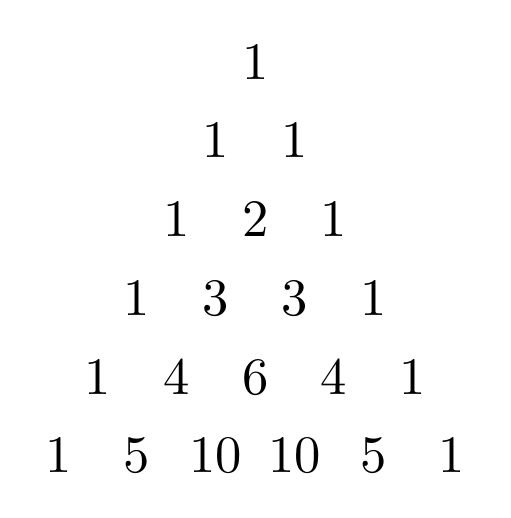
\begin{tikzpicture}[every node/.style={scale=1.9}]
    \draw(0,0) node {$1$};
    \draw(1,0) node {$5$};
    \draw(2,0) node {$10$};
    \draw(3,0) node {$10$};
    \draw(4,0) node {$5$};
    \draw(5,0) node {$1$};
    \draw(0.5,1) node {$1$};
    \draw(1.5,1) node {$4$};
    \draw(2.5,1) node {$6$};
    \draw(3.5,1) node {$4$};
    \draw(4.5,1) node {$1$};
    \draw(1,2) node {$1$};
    \draw(2,2) node {$3$};
    \draw(3,2) node {$3$};
    \draw(4,2) node {$1$};
    \draw(1.5,3) node {$1$};
    \draw(2.5,3) node {$2$};
    \draw(3.5,3) node {$1$};
    \draw(2,4) node {$1$};
    \draw(3,4) node {$1$};
    \draw(2.5,5) node {$1$};
  \end{tikzpicture}
\end{document}
